\begin{figure}[H]
  \centering
  \pgfplotsset{
    scaled y ticks=false,
    scale only axis,
    legend style={at={(0,0.8)}, anchor=west, font=\tiny},
    xmin=7,
  }
  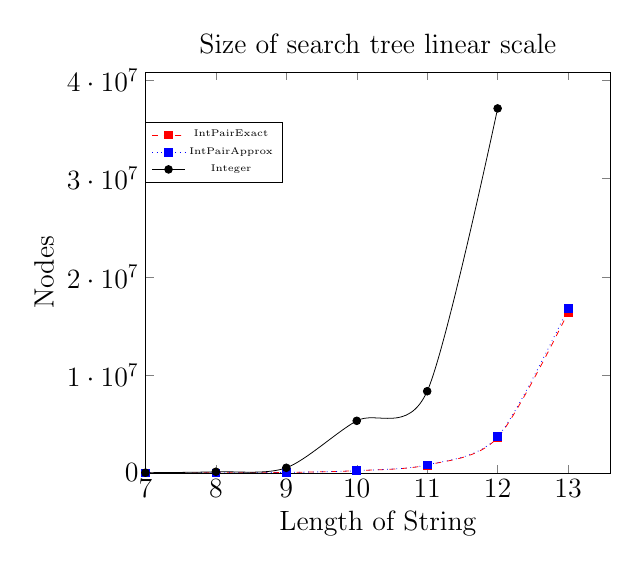
\begin{tikzpicture} [scale=0.7, font=\Large]
    \begin{axis}[
        title=Size of search tree linear scale,
        ylabel=Nodes,
        xtick=data,
        ymin=0, 
        xlabel=Length of String ]
      \addplot[smooth,mark=square*, mark options={solid},red, dashed]
      coordinates{ (7,2958) (8,12299) (9,53945) (10,233801) (11,809042) (12,3602055) (13,16361867)
      }; \label{ie_plot} \addlegendentry{IntPairExact}
      \addplot[smooth,mark=square*, mark options={solid},blue, dotted]
      coordinates{ (7,3048) (8,12623) (9,55211) (10,240131) (11,829618) (12,3696025) (13,16790307)
      }; \label{ia_plot} \addlegendentry{IntPairApprox}
      \addplot[smooth,mark=*,mark options={solid},black]
      coordinates{ (7, 28628) (8, 121116) (9, 527254) (10, 5315546) (11, 8329154) (12, 37151208)
      }; \label{int_plot} \addlegendentry{Integer}
    \end{axis}
  \end{tikzpicture}
  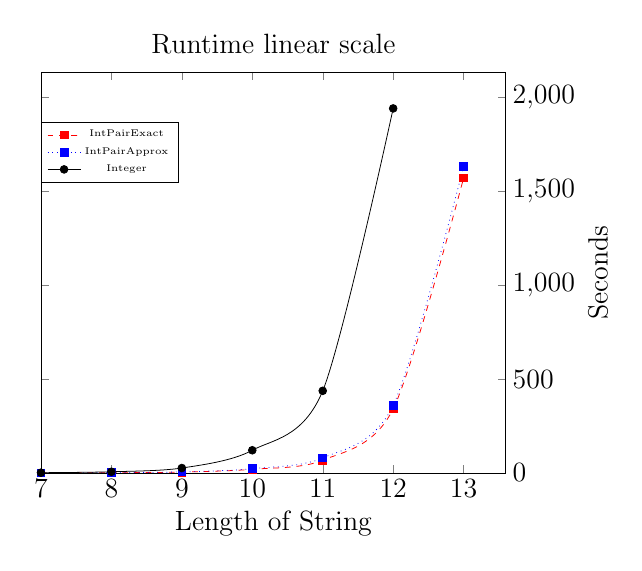
\begin{tikzpicture} [scale=0.7, font=\Large]
    \begin{axis}[
        yticklabel pos=right,
        xtick=data,
        title=Runtime linear scale,
        ylabel=Seconds,
        xlabel=Length of String,
        ymin=0, ]
      \addplot[smooth,mark=square*,mark options={solid},red, dashed]
      coordinates{ (7, .339) (8, 1.142) (9, 4.601) (10, 19.534) (11, 67.852) (12, 340.757) (13, 1569.780)
      }; \label{IntPairExact Run}
      \addplot[smooth,mark=square*,mark options={solid},blue, dotted]
      coordinates{ (7, .290) (8, 1.263) (9, 5.724) (10, 22.607) (11, 80.168) (12, 359.915) (13, 1629.885)
      }; \label{IntPairApprox Run}
      \addplot[smooth,mark=*,mark options={solid},black]
      coordinates{ (7, 1.464) (8,6.312) (9, 26.246) (10, 120.832) (11, 437.171) (12, 1940.096)
      }; \label{IntegerRun}
      \addlegendentry{IntPairExact}
      \addlegendentry{IntPairApprox}
      \addlegendentry{Integer}
    \end{axis}
  \end{tikzpicture}

  
\begin{tikzpicture}[scale=1.4]
    \draw[very thick] (-4,0) -- (4,0);
    \draw[draw=white] (-5,-0.2) -- (5,-0.2);
  \end{tikzpicture}


  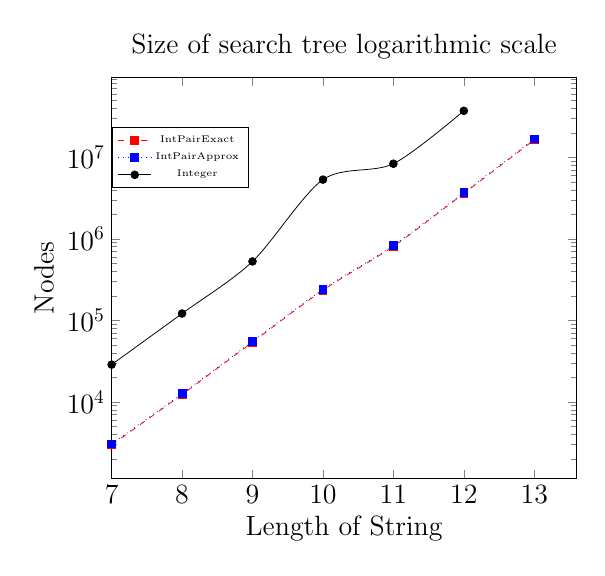
\begin{tikzpicture} [scale=0.7, font=\Large]
    \begin{semilogyaxis}[
        title=Size of search tree logarithmic scale,
        ylabel=Nodes,
        xtick=data,
        ymin=0, 
        xlabel=Length of String ]
     \addplot[smooth,mark=square*, mark options={solid},red, dashed]
      coordinates{ (7,2958) (8,12299) (9,53945) (10,233801) (11,809042) (12,3602055) (13,16361867)
      }; \label{ie_plot} \addlegendentry{IntPairExact}
      \addplot[smooth,mark=square*, mark options={solid},blue, dotted]
      coordinates{ (7,3048) (8,12623) (9,55211) (10,240131) (11,829618) (12,3696025) (13,16790307)
      }; \label{ia_plot} \addlegendentry{IntPairApprox}
      \addplot[smooth,mark=*,mark options={solid},black]
      coordinates{ (7, 28628) (8, 121116) (9, 527254) (10, 5315546) (11, 8329154) (12, 37151208)
      }; \label{int_plot} \addlegendentry{Integer}

    \end{semilogyaxis}
  \end{tikzpicture}
  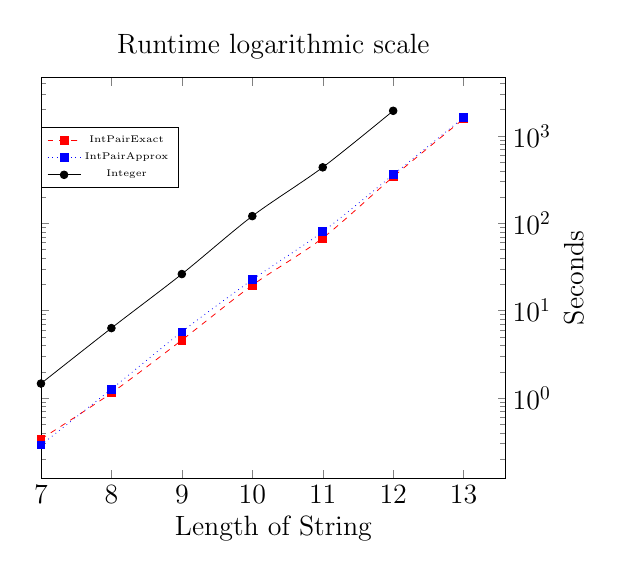
\begin{tikzpicture} [scale=0.7, font=\Large]
    \begin{semilogyaxis}[
        title=Runtime logarithmic scale,
        yticklabel pos=right,
        xtick=data,
        ylabel=Seconds,
        xlabel=Length of String,
        ymin=0,  ]
      \addplot[smooth,mark=square*,mark options={solid},red, dashed]
      coordinates{ (7, .339) (8, 1.142) (9, 4.601) (10, 19.534) (11, 67.852) (12, 340.757) (13, 1569.780)
      }; \label{IntPairExact Run}
      \addplot[smooth,mark=square*,mark options={solid},blue, dotted]
      coordinates{ (7, .290) (8, 1.263) (9, 5.724) (10, 22.607) (11, 80.168) (12, 359.915) (13, 1629.885)
      }; \label{IntPairApprox Run}
      \addplot[smooth,mark=*,mark options={solid},black]
      coordinates{ (7, 1.464) (8,6.312) (9, 26.246) (10, 120.832) (11, 437.171) (12, 1940.096)
      }; \label{IntegerRun}
      \addlegendentry{IntPairExact}
      \addlegendentry{IntPairApprox}
      \addlegendentry{Integer}
    \end{semilogyaxis}
  \end{tikzpicture}
%  \input{}
%\end{figure}
  \caption{Varying the length of the string. The other parameters are fixed. Number of states=7, size of alphabet=7, and max cost per transition=15. Here we also show graphs in logarithmic scale. The integer variable timed out for $steps=13$.}\label{fig:steps}
 \end{figure}
